\section{HTTP}

\begin{defi}{HTTP}
    \begin{center}
        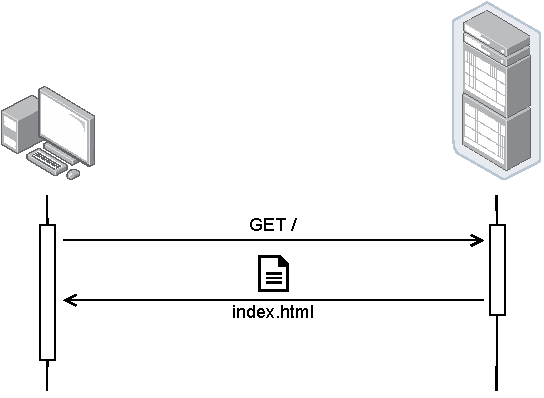
\includegraphics[width=0.5\textwidth]{includes/figures/defi_http.pdf}
    \end{center}

    Das \emph{Hypertext Transfer Protocol (HTTP)} ist ein textbasiertes, zustandsloses Anfrage-/Antwort-Protokoll der ISO/OSI-Schichten 5 bis 7.

    Es dient zur Übertragung von Datenobjekten zwischen einem Server und einem Client.
    Der Client sendet einen \emph{HTTP-Request} über eine aufgebaute TCP/IP-Verbindung an den Server.
    Dieser antwortet mit einer \emph{HTTP-Response}

    Der Endpunkt wird über eine URL identifiziert:

    \begin{center}
        \texttt{<protokoll>://<host>:<port>/<path>?<parameter>}
    \end{center}

    Beim Verbindungsaufbau fängt der Client an, in einer niedrigen \texttt{HTTP}-Version zu kommunizieren.
    Sobald er merkt, dass der Server Anfragen bearbeiten kann, erhöht er die \texttt{HTTP}-Version, bis er entweder keine Antwort erhält, oder selber keine neuere Version hat.
\end{defi}

\begin{defi}{URI}
    Ein \emph{Uniform Ressource Identifier (URI)} dient der eindeutigen Adressierung von abstrakten und physikalischen Ressourcen im Internet.

    URIs werden in zwei Gruppen aufgeteilt:
    \begin{itemize}
        \item \emph{Uniform Resource Location (URL)}
              \begin{itemize}
                  \item Benennen eine Ressource über ihren primären Zugriffsmechanismus wie zum Beispiel \texttt{http} oder \texttt{ftp}.
                  \item Danach folgt die Bezeichnung des Ortes (\emph{Location}) der Ressource im Netz – meistens der Domain-Name.\footnote{URLs waren ursprünglich die einzige Art von URIs, weshalb der Begriff URL oft gleichbedeutend mit URI verwendet wird.}
              \end{itemize}
        \item \emph{Uniform Ressource Name (URN)}:
              \begin{itemize}
                  \item Mit dem URI-Schema \texttt{urn} identifizieren eine Ressource mittels eines vorhandenen oder frei zu vergebenden Namens, beispielsweise \texttt{urn:isbn} oder \texttt{urn:sha1}.
              \end{itemize}
    \end{itemize}
\end{defi}

\begin{defi}{Klassische Client-Server-Architektur}
    \emph{Server} sind langlebige Prozesse, welche auf Anfragen von Clients warten und diese abarbeiten.

    \emph{Clients} stellen zu beliebigen Zeiten Anfragen und warten auf die Antwort.
    Die Rolle ist damit zumeist beendet.

    \begin{center}
        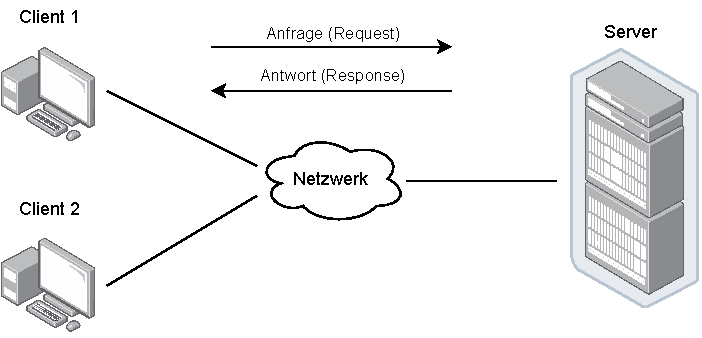
\includegraphics[width=0.75\textwidth]{includes/figures/defi_client_server.pdf}
    \end{center}
\end{defi}

\begin{bonus}{Dienst}
    Ein \emph{Dienst} wird von einem Verbund von Servern erbracht, durch den sich erst die Gesamtsicht ergibt.
    Ggf. merkt der Client nichts von dem Verbund.

    \begin{center}
        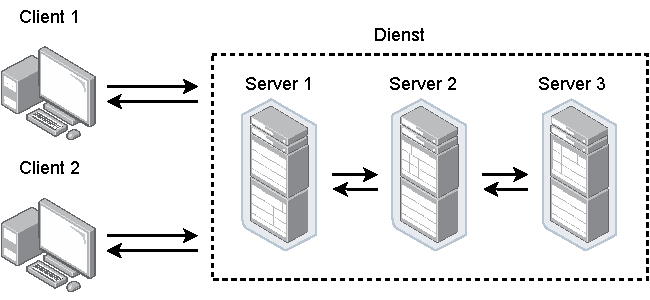
\includegraphics[width=0.6\textwidth]{includes/figures/bonus_dienst.pdf}
    \end{center}
\end{bonus}

\begin{bonus}{Proxy}
    Ein \emph{Proxy} dient zum Zwischenspeichern oder Anonymisieren von Anfragen auf der Clientseite, oder zum Lastbalanzieren auf der Serverseite.

    \begin{minipage}[t]{.5\textwidth}
        Forward Proxy:
    \end{minipage}%
    \begin{minipage}[t]{.5\textwidth}
        Reverse Proxy:
    \end{minipage}

    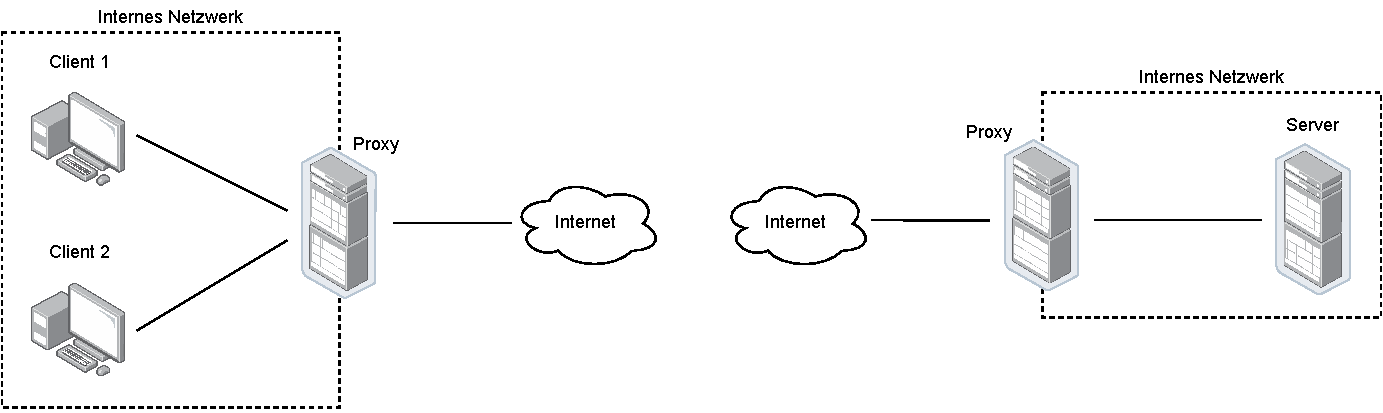
\includegraphics[width=\textwidth]{includes/figures/bonus_proxy.pdf}
\end{bonus}

\begin{defi}{CDN}
    \emph{Content Delivery Networks (CDN)} bieten Dienste an, um Inhalte auf multiple Server zu replizieren.
    Dies wird genutzt, da große Anbieter \enquote{nahe} beim Nutzenden sein wollen.

    Clients können so den Server nutzen, der den Inhalt am schnellsten liefert.
    Der Inhalt wird von einem Origin-Server geklont.

    \begin{center}
        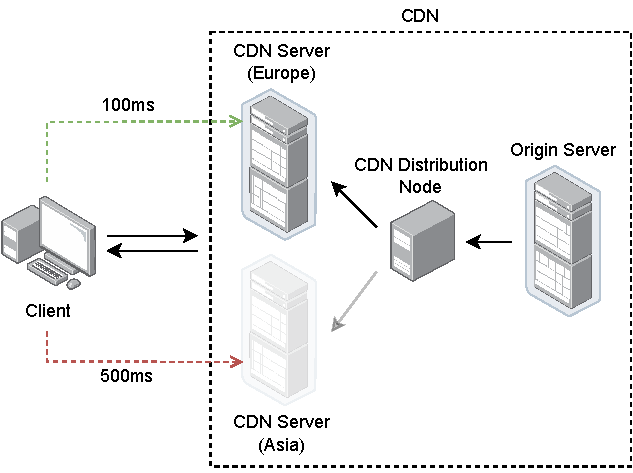
\includegraphics[width=0.5\textwidth]{includes/figures/defi_cdn.pdf}
    \end{center}
\end{defi}

\begin{defi}{HTTP-Request}
    \centering
    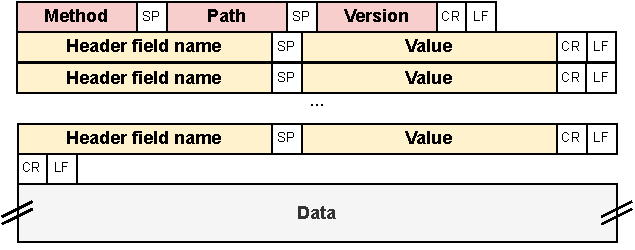
\includegraphics[width=0.75\textwidth]{includes/figures/defi_http_request_header.pdf}
\end{defi}

\begin{defi}{HTTP-Response}
    \centering
    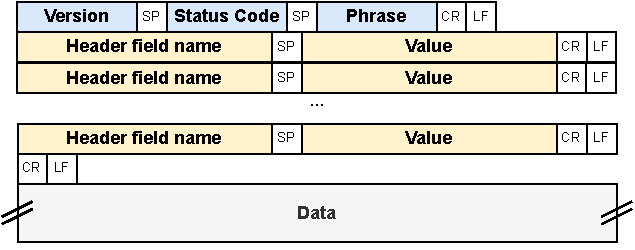
\includegraphics[width=0.75\textwidth]{includes/figures/defi_http_response_header.pdf}
\end{defi}

\begin{example}{HTTP Request inkl. Response}
    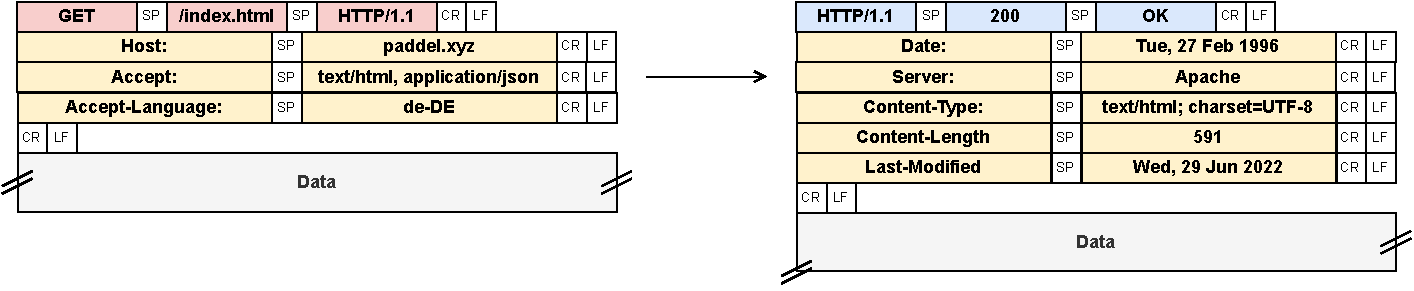
\includegraphics[width=\textwidth]{includes/figures/example_http_header.pdf}
\end{example}

\begin{bonus}{HTTP-Statuscode}
    \begin{center}
        \begin{tabular}{|c|l|l|}
            \hline
            Code         & Bedeutung     & Beschreibung                                             \\\hline\hline
            \texttt{1xx} & Informational & Anforderung empfangen, Aktion folgt                      \\\hline
            \texttt{2xx} & Success       & Erfolgreiche Abarbeitung der Anfrage                     \\\hline
            \texttt{3xx} & Redirection   & Angefragtes Objekt befindet sich an einer anderen Stelle \\\hline
            \texttt{4xx} & Client Error  & Falsche bzw. unerlaubte Anfrage                          \\\hline
            \texttt{5xx} & Server Error  & Server kann Anfrage nicht ausführen                      \\\hline
        \end{tabular}
    \end{center}
\end{bonus}

\begin{example}{HTTP-Statuscode}
    \begin{center}
        \begin{tabular}{|c|l|}
            \hline
            Code         & Bedeutung             \\\hline\hline
            \texttt{200} & OK                    \\\hline
            \texttt{301} & Moved Permanently     \\\hline
            \texttt{302} & Moved Temporarily     \\\hline
            \texttt{404} & Not Found             \\\hline
            \texttt{500} & Internal Server Error \\\hline
        \end{tabular}
    \end{center}
\end{example}

\begin{defi}{HTTP-Methoden}
    \begin{itemize}
        \item \texttt{GET} fordert eine Ressource an.
        \item \texttt{POST} schickt Daten zur weiteren Verarbeitung zum Server.
        \item \texttt{HEAD} weist den Server an, die gleichen HTTP-Header wie bei \texttt{GET}, nicht jedoch den Nachrichtenrumpf mit dem eigentlichen Dokumentinhalt zu senden.
        \item \texttt{PUT} dient dazu, eine Ressource unter Angabe des Ziel-URIs auf einen Webserver hochzuladen.
        \item \texttt{PATCH} ändert ein bestehendes Dokument ohne dieses wie bei PUT vollständig zu ersetzen.
        \item \texttt{DELETE} löscht die angegebene Ressource auf dem Server.
        \item \texttt{TRACE} liefert die Anfrage so zurück, wie der Server sie empfangen hat.
        \item \texttt{OPTIONS} liefert eine Liste der vom Server unterstützten Methoden und Merkmale.
        \item \texttt{CONNECT} wird von Proxyservern implementiert, die in der Lage sind, SSL-Tunnel zur Verfügung zu stellen.
    \end{itemize}
\end{defi}

\begin{defi}{GET (HTTP)}
    Bei \emph{GET}-Methoden werden die Daten über die Adresszeile übertragen.

    Sie sind sind nicht geeignet zur Übertragung großer Datenmengen.
\end{defi}

\begin{example}{GET (HTTP)}
    \begin{lstlisting} 
        GET /pokemon?^id=4^&^name=glumanda^
        HOST: paddel.xyz
    \end{lstlisting}
\end{example}

\begin{defi}{POST (HTTP)}
    Bei \emph{POST}-Methoden werden die Daten im HTTP-Body übertragen.
\end{defi}

\begin{example}{POST (HTTP)}
    \begin{lstlisting} 
        POST /pokemon
        HOST: paddel.xyz

        ^id=4^&^name=glumanda^
    \end{lstlisting}
\end{example}

\begin{example}{POST (HTML-Formular)}
    \begin{lstlisting}[language=HTML5]
        <form action="pokemon" method="post">
            <input type="number" name="id" />
            <input type="text" name="name" />
            <button type="submit"> show </button>
        </form>
    \end{lstlisting}

    Wird beim Absenden der Form übersetzt zu:

    %[language=HTTP]
    \begin{lstlisting}
        POST /pokemon
        HOST: paddel.xyz

        ^id=4^&^name=glumanda^
    \end{lstlisting}
\end{example}

\begin{bonus}{HTTP-Versionen}
    In den neueren Versionen von HTTP versucht man die Anzahl bzw. Dauer von weiteren Anfragen zu verhindern bzw. zu reduzieren.

    Während bei \emph{HTTP/1.1} noch jede Ressource einzeln abgefragt wurde, konnte man bei dem ursprünglichen \emph{HTTP/2.0} alle Dokumente gleichzeitig anfragen, die in dem ursprünglichen Dokument verknüpft wurden; z. B.:

    \emph{HTTP/1.1}: \texttt{GET index.html -> GET style.css -> GET script.js}

    \emph{HTTP/2.0}: \texttt{GET index.html -> GET style.css,  script.js}

    In neueren Version von \emph{HTTP/2.x} sendet der Server direkt Dateien mit, die der Client eventuell benötigen könnten.

    Der Client muss also nicht mehr alle Objekte selbständig anfragen.

    Bei dieser \emph{Push}-Variante können zwar \enquote{zu viele} Dateien mitgesendet werden, jedoch ist solch ein geringer Overhead bei aktuellen Netzwerkkapazitäten verkraftbar.
\end{bonus}